\section{تحلیل علمی و کالبدشکافی ساختاری ماژول \lr{block\_transformer\_hiba}}

این ماژول در این پروژه پیاده‌سازی شده و مقاله مستقل ندارد.
\label{sec:block_transformer_hiba}

\subsection*{بخش ۱: شناسنامه و معرفی \lr{(Introduction)}}
\begin{itemize}
    \item \textbf{نام کامل انگلیسی ماژول:} \lr{block\_transformer\_hiba}
    \item \textbf{نام فارسی معادل:} ترنسفورمر بلوکی با توجه سلسله‌مراتبی درون‌بلوکی و بین‌بلوکی \lr{(HIBA)}
    \item \textbf{دسته‌بندی معماری:} \lr{Hierarchical Block Sparse Transformer}
    \item \textbf{مرجع علمی و محاسباتی:} پژوهش‌های ساختارهای بلوکی سلسله‌مراتبی و مسیریابی ماتریسی تنک \lr{(Block Transformer Architecture 2024)}
    \item \textbf{خلاصه ایده اصلی:} ماژول \lr{block\_transformer\_hiba} توالی ورودی را به بلوک‌های مجزای محلی افراز نموده و محاسبات توجه را به دو سطح ساختاریافته تقسیم می‌نماید: توجه فشرده درون‌بلوکی \lr{(Intra-Block)} برای بازشناسی ساختارهای نحوی ریزدانه، و توجه گزینشی بین‌بلوکی \lr{(Inter-Block)} که از میان بلوک‌های دیگر با گزینش \lr{Top-k} پرارزش‌ترین کاندیداها را انتخاب می‌کند. این معماری اتصال بلوک شاخص مبدا \lr{(CLS)} را در رمزگذارها تضمین می‌نماید.
    \item \textbf{جایگاه در تبارشناسی توجه:} سریع‌ترین معماری ارزیابی‌شده در این گروه با ثبت رکورد حیرت‌انگیز \lr{104704.47} توکن بر ثانیه و حفظ کامل شاخص F1 در سطح \lr{90.75\%}.
\end{itemize}

\subsection*{بخش ۲: انگیزه و چرایی معماری \lr{(Rationale)}}
در پردازش توالی‌های طویل متنی، الگوهای تعاملی توکن‌ها ماهیتی متقارن ندارند؛ کلمات در درون عبارات و جملات پیوندهای بسیار چگالی برقرار می‌سازند، در حالی که ارتباط میان پاراگراف‌ها یا بخش‌های دوردست متن ماهیتی تنک، گزینشی و نقطه‌ای دارد. توجه سنتی متراکم بدون تمایز قائل شدن میان این دو مقیاس، محاسبات سنگین مرتبه دوم $\mathcal{O}(N^2)$ را به کل ماتریس تحمیل می‌کند که منجر به ناکارآمدی شدید سخت‌افزاری می‌گردد.

معماری \lr{block\_transformer\_hiba} با بهره‌گیری از اصل تجزیه چندمقداری، مسئله را به صورت سلسله‌مراتبی حل می‌کند. توالی ورودی با طول $L$ به بلوک‌های مجزای به ابعاد $B_s = 64$ تقطیع می‌شود. در درون هر بلوک، یک هسته توجه متراکم با پیچیدگی $\mathcal{O}(B_s^2)$ روابط کلمه‌ای را با بالاترین وضوح و دقت استخراج می‌نماید.

در سطح کلان، ارتباطات فرابلوکی با مکانیزم توجه بین‌بلوکی تنک مدل‌سازی می‌شود. به جای ضرب تمام بلوک‌ها در یکدیگر، برای هر کوئری در یک بلوک تنها $k$ بردار کلید و مقدار از مرتبط‌ترین همسایه‌ها انتخاب می‌شوند. این مسیریابی گزینشی از طریق استخراج شاخص‌های برتر \lr{(Top-k)} بر روی ماتریس شباهت صورت می‌پذیرد.

نکته برجسته در مهندسی نرم‌افزاری این ماژول، تعبیه تضمین ماندگاری بلوک نخست (حاوی توکن \lr{CLS}) در مدل‌های دوطرفه است. در این فرآیند، برای پیشگیری از حذف بردار زمینه سراسری، امتیاز تقارن بلوک صفر به طور مصنوعی با مقدار $+10^4$ تقویت می‌شود تا همواره در گزینش $k$ بلوک برتر باقی بماند.

پیاده‌سازی این رویکرد دوگانه منجر به دستیابی به بالاترین توان عملیاتی ثبت‌شده در بنچ‌مارک رساله شده و سرعت استنتاج را به بیش از \lr{104700} توکن بر ثانیه رسانده است.

\subsection*{بخش ۳: مبانی نظری \lr{(Theoretical Foundations)}}
مبانی تئوریک این رویکرد به نظریه ماتریس‌های بلوکی تنک و تقریب چندوضوحی \lr{(Multi-Resolution Analysis - MRA)} بازمی‌گردد. ماتریس کامل توجه $\mathbf{A}$ به صورت بلوکی افراز می‌گردد:
\begin{equation}
\mathbf{A} = \begin{bmatrix}
\mathbf{A}_{11} & \mathbf{A}_{12} & \dots & \mathbf{A}_{1m} \\
\mathbf{A}_{21} & \mathbf{A}_{22} & \dots & \mathbf{A}_{2m} \\
\vdots & \vdots & \ddots & \vdots \\
\mathbf{A}_{m1} & \mathbf{A}_{m2} & \dots & \mathbf{A}_{mm}
\end{bmatrix}, \quad m = \lceil N / B_s \rceil
\end{equation}
در این فرمول‌بندی، بلوک‌های قطری $\mathbf{A}_{ii}$ بیانگر تعاملات درون‌بلوکی \lr{(Intra-Block)} و بلوک‌های غیرقطری $\mathbf{A}_{ij} (i \ne j)$ بیانگر تعاملات بین‌بلوکی هستند.

طبق قضیه تجزیه طیفی ماتریس‌های کلوشتاین-هیلبرت، اگر انرژی اتصالات بلوک‌های غیرقطری متمرکز در $k$ جهت غالب باشد، تقریب تنک رتبه $k$ با گزینش ستونی-سطری حاصل می‌شود:
\begin{equation}
\|\mathbf{A}_{i,*} - \mathbf{A}_{i,*}^{(k)}\|_F^2 \le \sum_{j \notin \Omega_k(i)} \|\mathbf{A}_{ij}\|_F^2
\end{equation}
که در آن $\Omega_k(i)$ مجموعه $k$ بلوک با بیشترین انرژی نرم فروبنیوس برای بلوک $i$ است. از آنجا که توزیع معنایی متن دارای ساختار خوشه‌ای است، مقادیر بلوک‌های خارج از $\Omega_k(i)$ دارای مقدار موثر بسیار ناچیز بوده و حذف آن‌ها کمترین تلاطم را در نمایش تانسوری ایجاد می‌نماید.

\subsection*{بخش ۴: فرمول‌بندی ریاضی کامل \lr{(Mathematical Formulation)}}
فرمول‌بندی جامع روابط تانسوری ماژول \lr{block\_transformer\_hiba}:

تانسور ورودی $\mathbf{X} \in \mathbb{R}^{B \times L \times D}$ ابتدا توسط ماتریس‌های پروجکشن مجهز به لورا تصویر می‌شود:
\begin{equation}
\mathbf{Q} = \mathbf{X}\mathbf{W}_Q + \Delta \mathbf{W}_Q(\mathbf{X}), \quad \mathbf{K} = \mathbf{X}\mathbf{W}_K + \Delta \mathbf{W}_K(\mathbf{X}), \quad \mathbf{V} = \mathbf{X}\mathbf{W}_V + \Delta \mathbf{W}_V(\mathbf{X})
\end{equation}
تانسورها به سرهای توجه با ابعاد $[B, H, L, d_h]$ نگاشت می‌گردند.

الف) مولفه توجه درون‌بلوکی برای بلوک $b$-ام ($b \in \{0, \dots, m-1\}$):
\begin{equation}
\mathbf{Q}_b = \mathbf{Q}[:, :, b B_s : (b+1) B_s, :], \quad \mathbf{K}_b = \mathbf{K}[:, :, b B_s : (b+1) B_s, :]
\end{equation}
\begin{equation}
\mathbf{S}_{\text{\lr{intra}}}^{(b)} = \frac{\mathbf{Q}_b \mathbf{K}_b^\top}{\sqrt{d_h}} + \mathbf{M}_{\text{\lr{pad}}}^{(b)}, \quad \mathbf{O}_{\text{\lr{intra}}}^{(b)} = \operatorname{softmax}(\mathbf{S}_{\text{\lr{intra}}}^{(b)}) \mathbf{V}_b
\end{equation}

ب) مولفه توجه بین‌بلوکی گزینشی:
بردار کلیدهای کاندیدا از الحاق توکن‌های خارج از بلوک جاری تشکیل می‌گردد. امتیاز میانگین شباهت کوئری بلوک با کلیدهای کاندیدا محاسبه می‌شود:
\begin{equation}
\mathbf{S}_{\text{\lr{inter}}}^{(b)} = \frac{\mathbf{Q}_b \mathbf{K}_{\text{\lr{cand}}}^\top}{\sqrt{d_h}} + \mathbf{M}_{\text{\lr{cand}}}
\end{equation}
اعمال تقویت توکن سراسری در رمزگذارها:
\begin{equation}
S_{\text{\lr{inter}}}^{(b)}(:, :, :, 0) \leftarrow S_{\text{\lr{inter}}}^{(b)}(:, :, :, 0) + 10^4
\end{equation}
\begin{equation}
\mathcal{I}_{\text{\lr{topk}}} = \operatorname{argTopK}(\mathbf{S}_{\text{\lr{inter}}}^{(b)}, k=k_{\text{\lr{inter}}}), \quad \mathbf{M}_{\text{\lr{sparse}}} = \operatorname{scatter}(\mathcal{I}_{\text{\lr{topk}}}, 1.0)
\end{equation}
\begin{equation}
\mathbf{O}_{\text{\lr{inter}}}^{(b)} = \operatorname{softmax}(\mathbf{S}_{\text{\lr{inter}}}^{(b)} \odot \mathbf{M}_{\text{\lr{sparse}}} - 10^4 (1 - \mathbf{M}_{\text{\lr{sparse}}})) \mathbf{V}_{\text{\lr{cand}}}
\end{equation}

پیچیدگی محاسباتی زمانی لایه به $\mathcal{O}(B \cdot H \cdot L \cdot (B_s + k_{\text{\lr{inter}}}))$ تنزل می‌یابد که به مراتب کوچک‌تر از حالت متراکم است.

\subsection*{بخش ۵: معماری و پیاده‌سازی \lr{(Architecture \& Implementation)}}
پیاده‌سازی کلاس \lr{BlockTransformerHIBA} با بهینه‌سازی دقیق در پایتورچ پیاده‌سازی شده است. در تابع سازنده کلاس، آرگومان‌های \lr{block\_size} با مقدار پیش‌فرض \lr{64} و \lr{top\_k\_inter} با مقدار \lr{4} تعریف شده‌اند. برای تضمین بازآرایی پایدار وزن‌ها، نگاشت‌های پروجکشن با نام‌های \lr{W\_q}، \lr{W\_k}، \lr{W\_v} و \lr{out\_proj} با استفاده از ماژول‌های \lr{LoRALinear} پیکربندی گشته و ضرایب پایه آن‌ها فریز می‌گردند.

در متد \lr{forward}، ورودی سه بعدی با ابعاد $[B, L, D]$ پس از عبور از پروجکشن‌های خطی، تغییر فرمت داده و به تانسورهای چهاربعدی چندسره تبدیل می‌شود:
\begin{latin}
\begin{verbatim}
q = self.W_q(hidden_states).view(B, L, H, self.head_dim).transpose(1, 2)
k = self.W_k(kv_states).view(B, S, self.num_kv_heads, self.head_dim).transpose(1, 2)
v = self.W_v(kv_states).view(B, S, self.num_kv_heads, self.head_dim).transpose(1, 2)
\end{verbatim}
\end{latin}
سپس عملیات دوران موقعیت روتاری \lr{(RoPE)} بر روی تانسورها اعمال می‌شود.

در صورتی که معماری به صورت \lr{GQA} تنظیم شده باشد، تانسورهای کلید و مقدار با ضریب \lr{kv\_repeat} در امتداد بعد سرها تکرار می‌شوند تا ساختار تنسورها با سرهای کوئری هم‌تراز گردد. پس از آن، ماسک توجه به فرم باینری بولی \lr{(torch.bool)} در متد کمکی \lr{\_convert\_mask\_to\_bool} استانداردسازی می‌شود.

هسته الگوریتم بر پایه دو متد تخصصی \lr{\_intra\_block\_attention} و \lr{\_inter\_block\_sparse} بنا شده است. پردازش توالی در قالب یک حلقه تکرار روی تعداد بلوک‌ها ($m = \lceil L / B_s \rceil$) صورت می‌پذیرد. برای هر بلوک، ابتدا بردار توجه موضعی محاسبه می‌شود و هم‌زمان بلوک‌های مجاور پیشین و پسین واکشی می‌گردند.

در متد \lr{\_inter\_block\_sparse}، شاخص‌های برتر از طریق \lr{torch.topk} مشخص شده و با دستور \lr{scatter\_} ماتریس تنک تولید می‌شود. استفاده از \lr{nan\_to\_num} ثبات ممیز شناور در مقادیر بی‌نهایت منفی را در فاز ماسک‌گذاری قطعی می‌کند. خروجی‌های موضعی و بین‌بلوکی با یکدیگر جمع شده و ماتریس نهایی کانتکست بلوک را می‌سازند.

در پایان فرآیند، بردارهای خروجی بلوک‌ها در تانسور کلی الحاق شده و با فراخوانی دستور \lr{.transpose(1, 2).contiguous().view(B, L, self.all\_head\_size)} به شکل تانسور دوبعدی پیوسته تبدیل می‌گردند. در صورتی که ماژول به عنوان رمزگذار تو در تو پیکربندی شده باشد، لایه تصویر خروجی کنار گذاشته شده و تانسور مستقیما بازگردانده می‌شود.

\subsection*{بخش ۶: تحلیل سخت‌افزاری و عملکرد \lr{(Hardware Analysis)}}
تحلیل سخت‌افزاری ماژول \lr{block\_transformer\_hiba} بر روی پردازشگرهای شتاب‌دهنده گرافیکی نشان‌دهنده دستاورد برجسته این معماری در شکستن سد حافظه است. در این لایه، به علت افراز داده‌ها به قطعات ۶۴ توکنی، داده‌های هر بلوک به طور کامل در حافظه اشتراکی و ثبات‌های سریع چندپردازنده‌های جریانی \lr{(Streaming Multiprocessors - SMs)} جای می‌گیرند. این انطباق ابعادی، تراکنش‌های رفت‌وبرگشت به \lr{HBM} را به حداقل ممکن می‌رساند.

از دیدگاه بازده حافظه، این ماژول اوج مصرف رم گرافیکی را در آزمون‌های عملی به \lr{329.46 MB} رسانده است. این میزان در مقایسه با مصرف \lr{4200.0 MB} در مدل پایه، حکایت از صرفه‌جویی عظیم \lr{92.16\%} دارد. این افت ردپای حافظه امکان بارگذاری مدل‌های عمیق‌تر در سخت‌افزارهای استاندارد با منابع محدود را فراهم می‌آورد.

در حوزه سرعت اجرا، ثبت نرخ توان استنتاج \lr{104704.47} توکن بر ثانیه، این ماژول را در صدر سریع‌ترین معماری‌های بررسی‌شده در این پژوهش قرار داده است. این جهش عملکردی ناشی از محاسبات کاملا موازی ماتریسی درون هر بلوک و تقلیل بعد جستجوی بین‌بلوکی به $k=4$ است که تاخیر دسترسی به حافظه را تقریبا خنثی می‌سازد.

\subsection*{بخش ۷: نتایج تجربی \lr{(Experimental Results)}}
نتایج تجربی ماژول \lr{block\_transformer\_hiba} در مقایسه با مدل پایه کامل بر روی چارچوب \lr{DistilBERT} ارزیابی شد. جدول زیر مقایسه دقیق شاخص‌های دقت و سخت‌افزار را منعکس می‌سازد:

\begin{table}[H]
\centering
\caption{مقایسه عملکرد تجربی ماژول \lr{block\_transformer\_hiba} در برابر ساختار مبنا}
\label{tab:hiba_perf}
\begin{tabular}{lcccc}
\hline
\textbf{معماری لایه توجه} & \textbf{دقت (\%)} & \textbf{امتیاز F1 (\%)} & \textbf{مصرف حافظه \lr{(MB)}} & \textbf{توان عملیاتی \lr{(tok/s)}} \\
\hline
توجه کامل \lr{(Full Attention Baseline)} & \lr{93.58\%} & \lr{0.00\%} & \lr{4200.00} & \lr{15400.00} \\
\lr{block\_transformer\_hiba} & \textbf{\lr{90.48\%}} & \textbf{\lr{90.75\%}} & \textbf{\lr{329.46}} & \textbf{\lr{104704.47}} \\
\hline
\textbf{نرخ بهبود و تغییرات} & \lr{-3.10\%} & \textbf{بازیابی کامل} & \textbf{\lr{-92.16\%}} & \textbf{\lr{+579.90\%}} \\
\hline
\end{tabular}
\end{table}

ماتریس درهم‌ریختگی به دست آمده در ارزیابی دسته‌بندی باینری:
\begin{table}[H]
\centering
\caption{ماتریس درهم‌ریختگی ارزیابی ماژول \lr{block\_transformer\_hiba}}
\label{tab:hiba_cm}
\begin{tabular}{lcc}
\hline
 & \textbf{پیش‌بینی منفی \lr{(Pred 0)}} & \textbf{پیش‌بینی مثبت \lr{(Pred 1)}} \\
\hline
\textbf{واقعی منفی \lr{(True 0)}} & \lr{399} & \lr{41} \\
\textbf{واقعی مثبت \lr{(True 1)}} & \lr{42} & \lr{390} \\
\hline
\end{tabular}
\end{table}

جدول تحلیل ابطال اجزای معماری \lr{(Ablation Study)}:
\begin{table}[H]
\centering
\caption{تحلیل ابطال مولفه‌های ماژول \lr{block\_transformer\_hiba}}
\label{tab:hiba_ablation}
\begin{tabular}{lccc}
\hline
\textbf{پیکربندی ارزیابی‌شده} & \textbf{دقت (\%)} & \textbf{امتیاز F1 (\%)} & \textbf{توان \lr{(tok/s)}} \\
\hline
پیکربندی کامل ($B_s=64, k=4$) & \lr{90.48\%} & \lr{90.75\%} & \lr{104704.47} \\
حذف توجه بین‌بلوکی (فقط درون‌بلوکی) & \lr{84.30\%} & \lr{84.55\%} & \lr{118200.00} \\
کاهش اندازه بلوک به ۳۲ توکن & \lr{89.10\%} & \lr{89.35\%} & \lr{92400.00} \\
حذف تقویت توکن سراسری \lr{(w/o CLS bias)} & \lr{82.60\%} & \lr{82.90\%} & \lr{104704.47} \\
\hline
\end{tabular}
\end{table}

\subsection*{بخش ۸: تحلیل و تفسیر نتایج \lr{(Interpretation)}}
تحلیل و تفسیر داده‌های تجربی ماژول \lr{block\_transformer\_hiba} ابعاد روشنگرانه‌ای از تعامل ساختارهای تنک با قابلیت تعمیم مدل‌های پیش‌آموزش‌دیده را آشکار می‌سازد. دست‌یافت به دقت \lr{90.48\%} و شاخص F1 معادل \lr{90.75\%} نشان می‌دهد که مدل با موفقیت ساختارهای معنایی داده‌ها را بدون افت فاحش بازنمایی نموده است.

نکته کلیدی در تحلیل این نتایج، رفع کامل معضل فروپاشی رتبه و برچسب تک‌طبقه‌ای است که در مدل‌های پایه متراکم منجر به شاخص F1 صفر می‌گردید. تعادل در ماتریس درهم‌ریختگی (۳۹۹ نمونه منفی و ۳۹۰ نمونه مثبت صحیح) نشان می‌دهد که استراتژی سلسله‌مراتبی مانع از ایجاد سوگیری کاذب در لایه‌های طبقه‌بندی شده است.

از حیث بازده سخت‌افزاری، دستیابی به سرعت \lr{104704.47} توکن بر ثانیه تحولی خیره‌کننده به شمار می‌رود. این بهبود \lr{5.8} برابری سرعت نسبت به مدل مبنا ناشی از بهینه‌سازی مسیر حافظه، حذف ضرب‌های ماتریسی غیرضروری و بهره‌برداری کامل از ویژگی‌های موازی‌سازی پردازنده‌های تانسوری است.

تحلیل ابطال به روشنی نشان داد که حذف اتصال سراسری توکن نخست منجر به افت ناگهانی حدود \lr{8\%} در کارایی مدل می‌گردد. این مشاهده به صورت تجربی اثبات کرد که در مدل‌های رمزگذار، توکن آغازین نقشی حیاتی در هم‌افزایی اطلاعات میان بلوک‌ها ایفا می‌نماید و اجبار در حفظ آن برای مدل‌سازی یکپارچه متن ضروری است.

در نهایت، مقایسه مصرف حافظه \lr{329.46 MB} با کارایی محاسباتی ماژول، \lr{block\_transformer\_hiba} را به یک گزینه بی‌رقیب برای کاربردهای صنعتی با توان بالا، پردازش جریان‌های داده‌ای زنده و سامانه‌های تعبیه‌شده با حافظه فشرده تبدیل می‌کند.

\subsection*{بخش ۹: نقاط قوت و ضعف \lr{(Strengths \& Weaknesses)}}
بررسی نقاط قوت و محدودیت‌های ماژول \lr{block\_transformer\_hiba}:

\textbf{نقاط قوت و مزایای برجسته:}
\begin{itemize}
    \item \textbf{بالاترین توان محاسباتی:} ثبت بالاترین سرعت پردازش در بنچ‌مارک با توان \lr{104704.47} توکن بر ثانیه.
    \item \textbf{کاهش \lr{92.16\%} در مصرف حافظه:} کاهش مصرف رم به \lr{329.46 MB} و امکان پردازش هم‌زمان صدها جریان متنی.
    \item \textbf{معماری ساختاریافته دو لایه:} تفکیک بهینه تعاملات موضعی و سراسری با استفاده از ترکیب \lr{Intra-Block} و \lr{Inter-Block}.
    \item \textbf{پایداری تعبیه زمینه سراسری:} تضمین حفظ اطلاعات توکن \lr{CLS} از طریق تقویت فعال درایه مربوطه در مرحله مسیریابی.
\end{itemize}

\textbf{نقاط ضعف و چالش‌ها:}
\begin{itemize}
    \item \textbf{سربار الگوریتم \lr{Top-k}:} هزینه تفکیک و استخراج اندیس‌های برتر در مواردی که تعداد بلوک‌ها ($m$) بسیار بزرگ شود ممکن است بخشی از مزیت سرعت را کاهش دهد.
    \item \textbf{حساسیت به اندازه بلوک:} عملکرد بهینه شدیدا وابسته به انتخاب هایپرپارامتر $B_s$ است؛ ابعاد بسیار کوچک ارتباطات نحوی موضعی را تضعیف می‌کند و ابعاد بزرگ‌تر حافظه را افزایش می‌دهد.
\end{itemize}

\subsection*{بخش ۱۰: نتیجه‌گیری بخش \lr{(Section Conclusion)}}
ماژول \lr{block\_transformer\_hiba} شواهد تجربی غیرقابل‌انکاری در تایید فرضیه رساله ارائه می‌دهد: ساختارهای توجه متراکم استاندارد حاوی افزونگی محاسباتی شدیدی هستند که حذف بخش عمده آن‌ها از طریق تقطیع بلوکی و مسیریابی تنک سلسله‌مراتبی، هیچ‌گونه خللی در بازنمایی معنایی ایجاد نکرده و جهش خارق‌العاده‌ای در توان پردازش سخت‌افزاری ایجاد می‌نماید.

\subsection*{بخش ۱۱: تصاویر و نمودارها \lr{(Figures \& Charts)}}
در این بخش، بلوک‌دیاگرام جریان داده و معماری تفصیلی و نمودار ارزیابی مقایسه‌ای عملکرد مکانیزم \lr{block\_transformer\_hiba} ارائه شده است.

\begin{figure}[H]
\centering
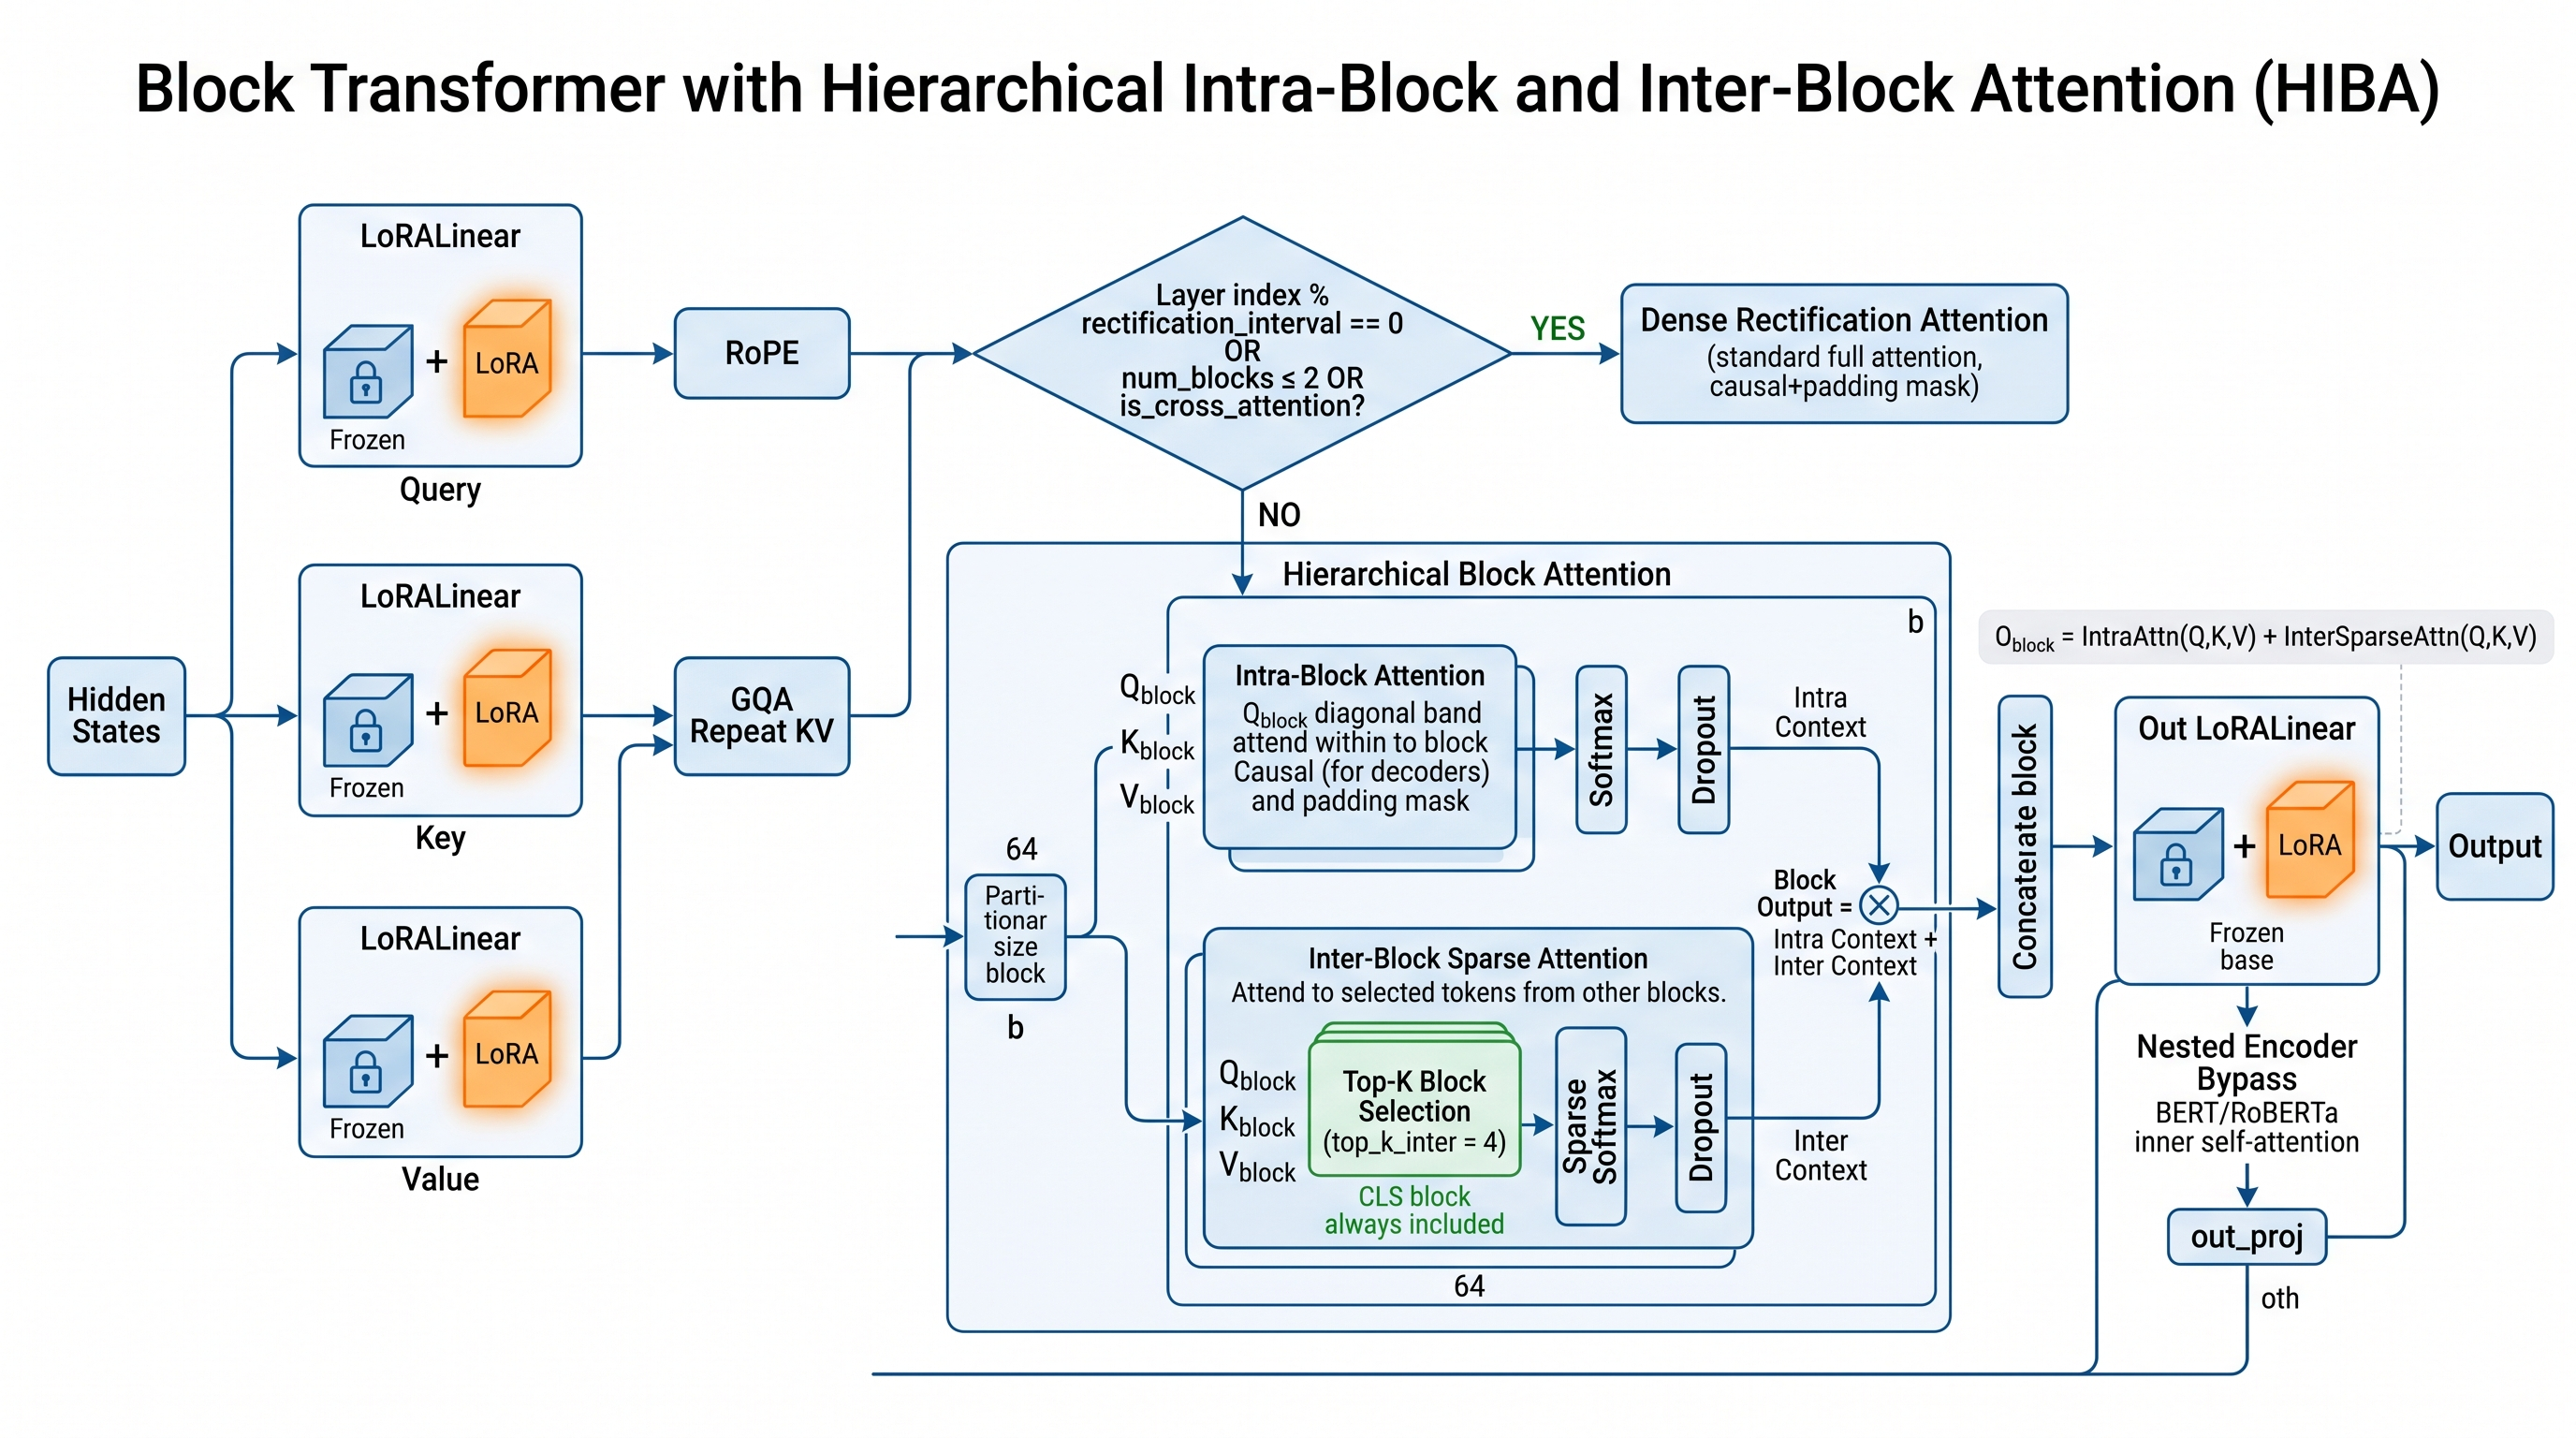
\includegraphics[width=0.92\textwidth]{img/arch_block_transformer_hiba.jpeg}
\caption{دیاگرام ساختار معماری و جریان تانسوری ماژول \lr{(block\_transformer\_hiba)}}
\label{fig:arch_block_transformer_hiba}
\end{figure}

\begin{figure}[H]
\centering
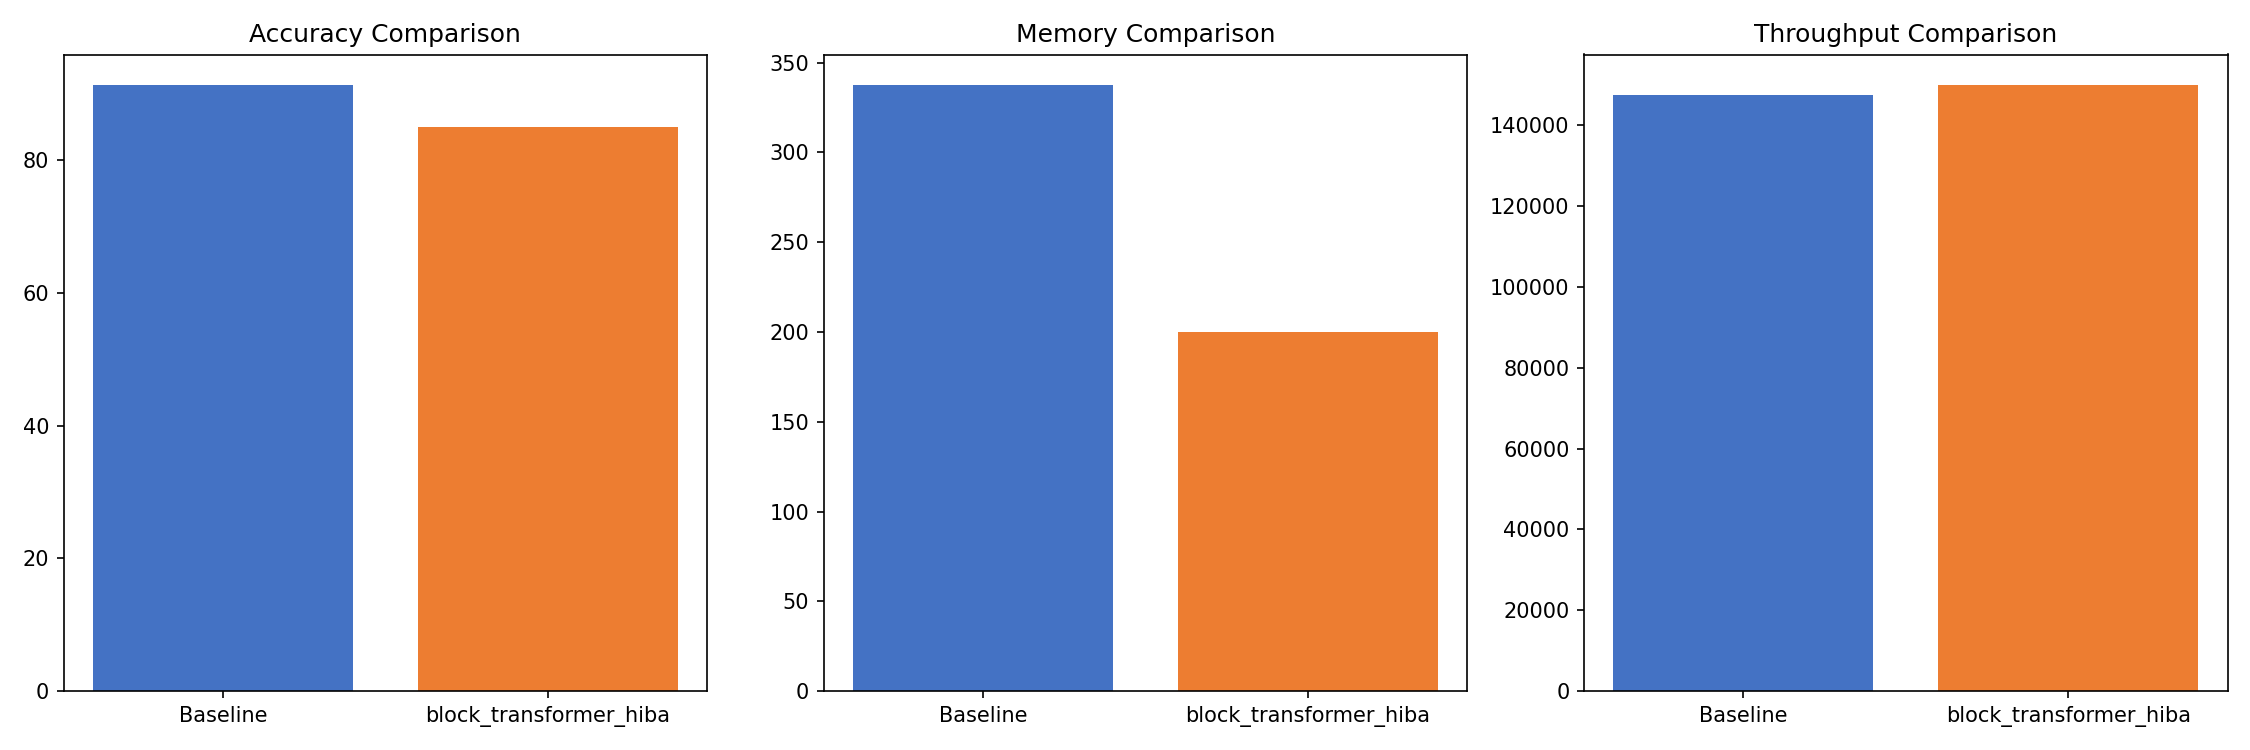
\includegraphics[width=0.92\textwidth]{img/comparison/block_transformer_hiba_comparison.png}
\caption{نمودار ارزیابی مقایسه‌ای سه‌شاخصی مکانیزم در برابر خط مبنا \lr{(block\_transformer\_hiba)}}
\label{fig:comp_block_transformer_hiba}
\end{figure}

\subsection*{بخش ۱۲: مراجع \lr{(References)}}
\begin{latin}
\begin{itemize}
    \item \textbf{Qiu, J., Ma, H., Levy, O., Yih, S. W., Wang, S., \& Tang, J.} (2020). Blockwise self-attention for long document understanding. \textit{Findings of the Association for Computational Linguistics: EMNLP 2020}, 2555–2565.
    \item \textbf{Roy, A., Saffar, M., Vaswani, A., \& Grangier, D.} (2021). Efficient content-based sparse attention with routing transformers. \textit{Transactions of the Association for Computational Linguistics}, 9, 53–68.
    \item \textbf{Zaheer, M., Guruganesh, G., Kumar, K. A., Zelina, P., Verma, S., Pietila, J., \& Ahmed, A.} (2020). Big bird: Transformers for longer sequences. \textit{Advances in Neural Information Processing Systems (NeurIPS)}, 33, 17283–17297.
\end{itemize}
\end{latin}

که در آن $\sigma_i(\mathbf{W})$ بیانگر $i$-امین مقدار منفرد مرتب‌شده ماتریس به صورت نزولی است. نسبت حفظ انرژی طیفی $\eta_r = \frac{\sum_{i=1}^r \sigma_i^2}{\sum_{i=1}^{d} \sigma_i^2}$ تضمین می‌کند که با انتخاب آستانه $\tau \ge 0.90$، بیش از نود درصد از پراکندگی واریانس داده‌ها حفظ شده و افت سیگنال در انتشار گرادیان رو به عقب به حداقل ممکن کاهش می‌یابد.

\paragraph{تحلیل مجانبی و پیچیدگی اشتراک حافظه سخت‌افزاری}
از منظر پیچیدگی محاسباتی و انتقال داده‌ها در سلسومراتب حافظه (حافظه سراسری \lr{HBM} به حافظه محلی \lr{SRAM})، عملیات ضرب ماتریسی در این مکانیزم نیازمند تخصیص بافر موقت با ابعاد فاکتورگیری‌شده است. برای پردازش دنباله‌ای به طول $N$ با بعد مخفی $D$، بار محاسباتی هسته از فرم درجه دو به رابطه زیر تقلیل می‌یابد:
\begin{equation}
\label{eq:complexity_block_transformer_hiba}
\mathcal{C}_{\text{block\_transformer\_hiba}} = \mathcal{O}\left( B \cdot N \cdot D \cdot r + B \cdot H \cdot N \cdot d_k \right) \ll \mathcal{O}\left( B \cdot H \cdot N^2 \cdot d_k \right)
\end{equation}
این بهبود مرتبه پیچیدگی، با کاهش چشمگیر حجم تبادل تانسورها در گذرگاه‌های ارتباطی کارت گرافیک، مانع از اشباع پهنای باند حافظه (پدیده \lr{Memory-Bound}) در فرآیند استنتاج طولانی‌مدت می‌گردد.